\section{Créer un lien vers une ressource extérieure.}
Il peut être pratique de conserver sous forme de fichier un lien vers une ressource internet. 
Dans mon établissement ce type de fichier m'est très pratique pour déployer sur tous les postes accueillant les évaluations des élèves de 6\ieme{} en utilisant un fichier sur un espace de stockage partagé en interne dans l'établissement et en le copiant de poste en poste --nous n'avons pas de domaine, ni de politique de déploiement par GPO-- du coup le fichier \texttt{.url} contient le lien qui sera ouvert par le navigateur par défaut de la machine vers le site web de passation des épreuves. 

%\newpage % force le passage sur une nouvelle page pour que les colonnes restent bien comme il faut, au besoin
\begin{multicols}{2}
Tout commence par le menu $\oplus$ \ldots
\begin{figure}
	\centering
	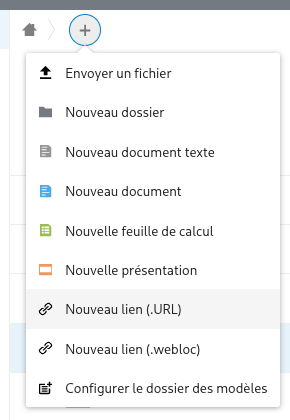
\includegraphics{./Captures/nuage.menu.plus.zoom.png}
	\caption{Le menu $\oplus$.}
\end{figure}
\columnbreak

Je sélection la ligne pour les URL.
\begin{figure}
	\centering
	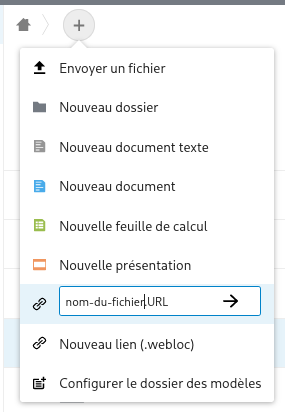
\includegraphics{./Captures/nuage.menu.plus.creer.url.png}
	\caption{Nommage du raccourcis}
\end{figure}
\end{multicols}

Je choisis de nommer par \texttt{nom-du-fichier} le fichier \texttt{.URL} qui sera généré, il contiendra un lien vers le site \url{https://ctan.org}~:
\begin{figure}
	\centering
	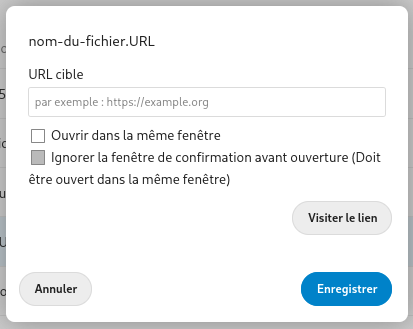
\includegraphics[width=0.333\linewidth]{./Captures/nuage.url.proprietes.png}
	\caption{Les propriétés du lien.}
\end{figure}

et je règle les options relatives à son ouverture (même fenêtre, fenêtre de confirmation, \ldots), ce qui fait qu'en cliquant sur le lien, la mini fenêtre suivante va s'afficher :
\begin{figure}
	\centering
	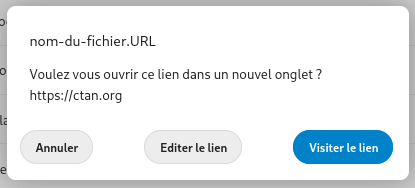
\includegraphics[width=0.333\linewidth]{./Captures/nuage.url.fenetre.confirmation.png}
	\caption{Confirmation de l'ouverture du lien.}
\end{figure}

Le site s'ouvre alors dans un nouvel onglet conformément aux propriétés réglées antérieurement.
\begin{figure}
	\centering
	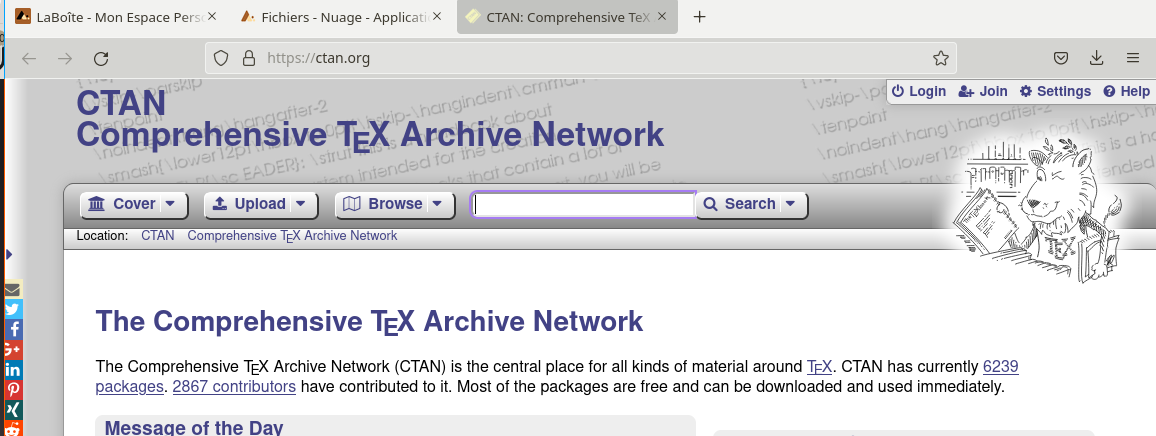
\includegraphics{./Captures/nuage.url.ouverture.nouvel.onglet.png}
	\caption{Le site CTAN.org est désormais ouvert dans un nouvel onglet.}
\end{figure}